\section{Experiment Details}
\label{appendix:exp_details}

\subsection{Models and Configuration}
\label{appendix:model_details}

\paragraph{API Access} We access all models from the Gemini-3 family (\texttt{gemini-3.1-pro-preview}, \texttt{gemini-\\3-flash-preview}, and \texttt{gemini-3-pro-image-preview}) via the Google Cloud Vertex AI platform. The GPT model (\texttt{gpt-5-2025-08-07}) is accessed via the official OpenAI API. Paper searches for verification and metadata fetching are conducted using the Semantic Scholar API (\url{https://api.semanticscholar.org/graph/v1/paper/search}).

\paragraph{Model Usage} The primary manuscript writing backbone for \ourmethod{} and all baselines is strictly fixed to Gemini-3.1-Pro. For literature discovery, \ourmethod{} utilizes Gemini-3-Flash with Google Search grounding. To ensure a fair comparison, we also use Gemini-3-Flash for the citation gathering process in AI Scientist-v2.

\paragraph{Evaluation Settings} For automated technical quality evaluations (AgentReview~\citep{jin2024agentreview}, AI Scientist-v2 Reviewer~\citep{yamada2025aiscientistv2}, and ScholarPeer~\citep{goyal2026scholarpeer}), we apply a universal temperature of 0.75 (Gemini-3.1-Pro) to balance instruction adherence with creative synthesis. For automated side-by-side evaluations, Gemini-3.1-Pro is set to a temperature of 0.0 to guarantee reproducibility. Since GPT-5 does not currently support temperature adjustment, we operate it at its fixed default temperature of 1.0 across all evaluations. During ScholarPeer~\citep{goyal2026scholarpeer} evaluation, we disable the baseline scouting agent for all pipelines to isolate presentation quality from fixed experimental constraints.

\paragraph{Research Cutoff} We align the research cutoff dates with the official submission deadlines of each venue: November 2024 for CVPR 2025 papers and October 2024 for ICLR 2025 papers.


\subsection{Baseline Selection}
\label{appendix:baseline_selection}

We explain why several existing systems are not included as baselines:

\begin{itemize}
    \item \textbf{OmniScientist}~\citep{shao2025omniscientist}: Lacks a publicly available, reproducible codebase.
    \item \textbf{PaperRobot}~\citep{wang2019paperrobot} and \textbf{Data-to-Paper}~\citep{technion2024datatopaper}: Do not support end-to-end generation of submission-ready \mylatex\ manuscripts.
    \item \textbf{AI-Researcher}~\citep{tang2025ai}: Operates as a full research pipeline requiring highly structured intermediate states (e.g., pre-written sections, curated literature summaries) rather than unconstrained raw materials. Adapting it to our setting would require reconstructing these abstractions, bypassing the core synthesis challenge our benchmark evaluates.
    \item \textbf{CycleResearcher}~\citep{weng2024cycleresearcher}: Requires a structured BibTeX reference list as input—an artifact rarely available during early drafting. The model also fails on unstructured inputs outside its specific training format, preventing it from directly processing raw materials.
    \item \textbf{Generic RAG pipelines} (\citep{wu2025autosurvey2}, \citep{go2025lira}): Designed primarily for literature surveys, these lack the specialized mechanisms required to autonomously draft, structure, and format full submission-ready research papers.
\end{itemize}

\subsection{Citation Verification}
\label{appendix:citation_verification}

To guarantee the factual accuracy and relevance of the generated literature review, our system employs a two-phase retrieval and verification pipeline for citation gathering. First, we use Gemini-3-Flash with Google Search grounding to rapidly discover candidate papers based on the generated outline. Following this discovery phase, each candidate paper undergoes strict sequential verification via the Semantic Scholar API to extract abstracts and metadata.

During verification, each candidate must resolve to a valid Semantic Scholar entity via a fuzzy title match (Levenshtein distance ratio $> 70$~\citep{Levenshtein1965BinaryCC}), augmented by a point-bonus for exact year alignment. To enter the final context pool, the entity must possess a retrievable abstract and strictly predate the research cutoff (when specified down to the month, the system defaults to the first day of that month as the strict boundary). Finally, gathered citations are deduplicated using unique paper ID keys.

Once the papers are verified and enriched with metadata (including authors, venue, year, citation count, and abstract), the compiled context is passed to the primary writing agent. To enforce high citation density and eliminate hallucinated references, the system prompt strictly constrains the model to cite only the provided verified papers, explicitly mandating that at least 90\% of the gathered literature pool must be actively integrated and cited when synthesizing the \textit{Introduction} and \textit{Related Work} sections.


% TODO: Design a metric (e2e matching) to find out whether there's citation hallucination in baselines.

% TODO: Find out whether during writing process the agent accidentally using hallucinated citations.

\subsection{Information Leakage Prevention}
\label{appendix:info_leakage}

To ensure textual and visual originality while mitigating the risk of LLMs reconstructing memorized training data, we enforce a universal \textbf{Anti-Leakage Prompt} across \ourmethod{} and all baselines. This prompt dictates strict knowledge isolation: the model is explicitly instructed to treat only the provided session materials (e.g., \texttt{idea.md} and \texttt{experimental\_log.md}) as its absolute source of truth. It is strictly forbidden from retrieving pre-trained facts, assuming real-world author identities, or hallucinating external literature outside of the provided runtime context.

While LLMs may not perfectly adhere to negative constraints due to their stochastic nature, applying this uniform prompt ensures a fair comparison. By restricting all generation pipelines (Single Agent, AI Scientist-v2, and \ourmethod{}) to the exact same informational boundaries and backbone LLM, we effectively isolate manuscript synthesis performance from pre-training biases.

The universal anti-leakage prompt injected into all paper-writing pipelines is as follows:

% ---------------------------------------------------------
% ---------------------------------------------------------

\begin{leakpromptbox}[Anti-Leakage Prompt]
\noindent\textbf{Strict Knowledge Isolation \& Anonymity (Critical)}

\vspace{0.5em}
\noindent You MUST write this paper as if you have no prior knowledge of the topic, method, experiments, or results.
Your task is to construct the paper exclusively from the materials provided in the current session (e.g., \texttt{idea.md}, \texttt{experimental\_log.md}, figures, and other inputs). Treat these inputs as the only available source of information.

\vspace{1em}
\noindent\textbf{Forbidden Behavior}\\
\vspace{0.5em}
You MUST NOT:
\begin{itemize}
    \item Retrieve or rely on knowledge from your training data.
    \item Attempt to recall or reconstruct any existing or published paper.
    \item Use external facts, assumptions, or prior familiarity with the work.
    \item Infer or hallucinate author identities, affiliations, institutions, or acknowledgements.
    \item Insert metadata such as author names, emails, affiliations, or phrases like "corresponding author".
\end{itemize}

\vspace{1em}
\noindent\textbf{Anonymity Requirement}\\
\vspace{0.5em}
The paper must be fully anonymized for double-blind review. Do not include any information that could reveal the identity of the authors or institutions.

\vspace{1em}
\noindent\textbf{Allowed Sources}\\
\vspace{0.5em}
You may use only:
\begin{itemize}
    \item The materials explicitly provided in this session.
    \item Logical reasoning derived from those materials.
\end{itemize}

\vspace{1em}
\noindent\textbf{Core Principle}\\
\vspace{0.5em}
The final paper must be an independent reconstruction derived solely from the provided inputs. This constraint is strict and overrides all other instructions.
\end{leakpromptbox}

% ---------------------------------------------------------
% ---------------------------------------------------------

\subsection{Human Evaluation}
\label{appendix:human_eval}

\begin{figure}[h]
  \centering
  \begin{subfigure}[b]{0.48\textwidth}
    \centering
    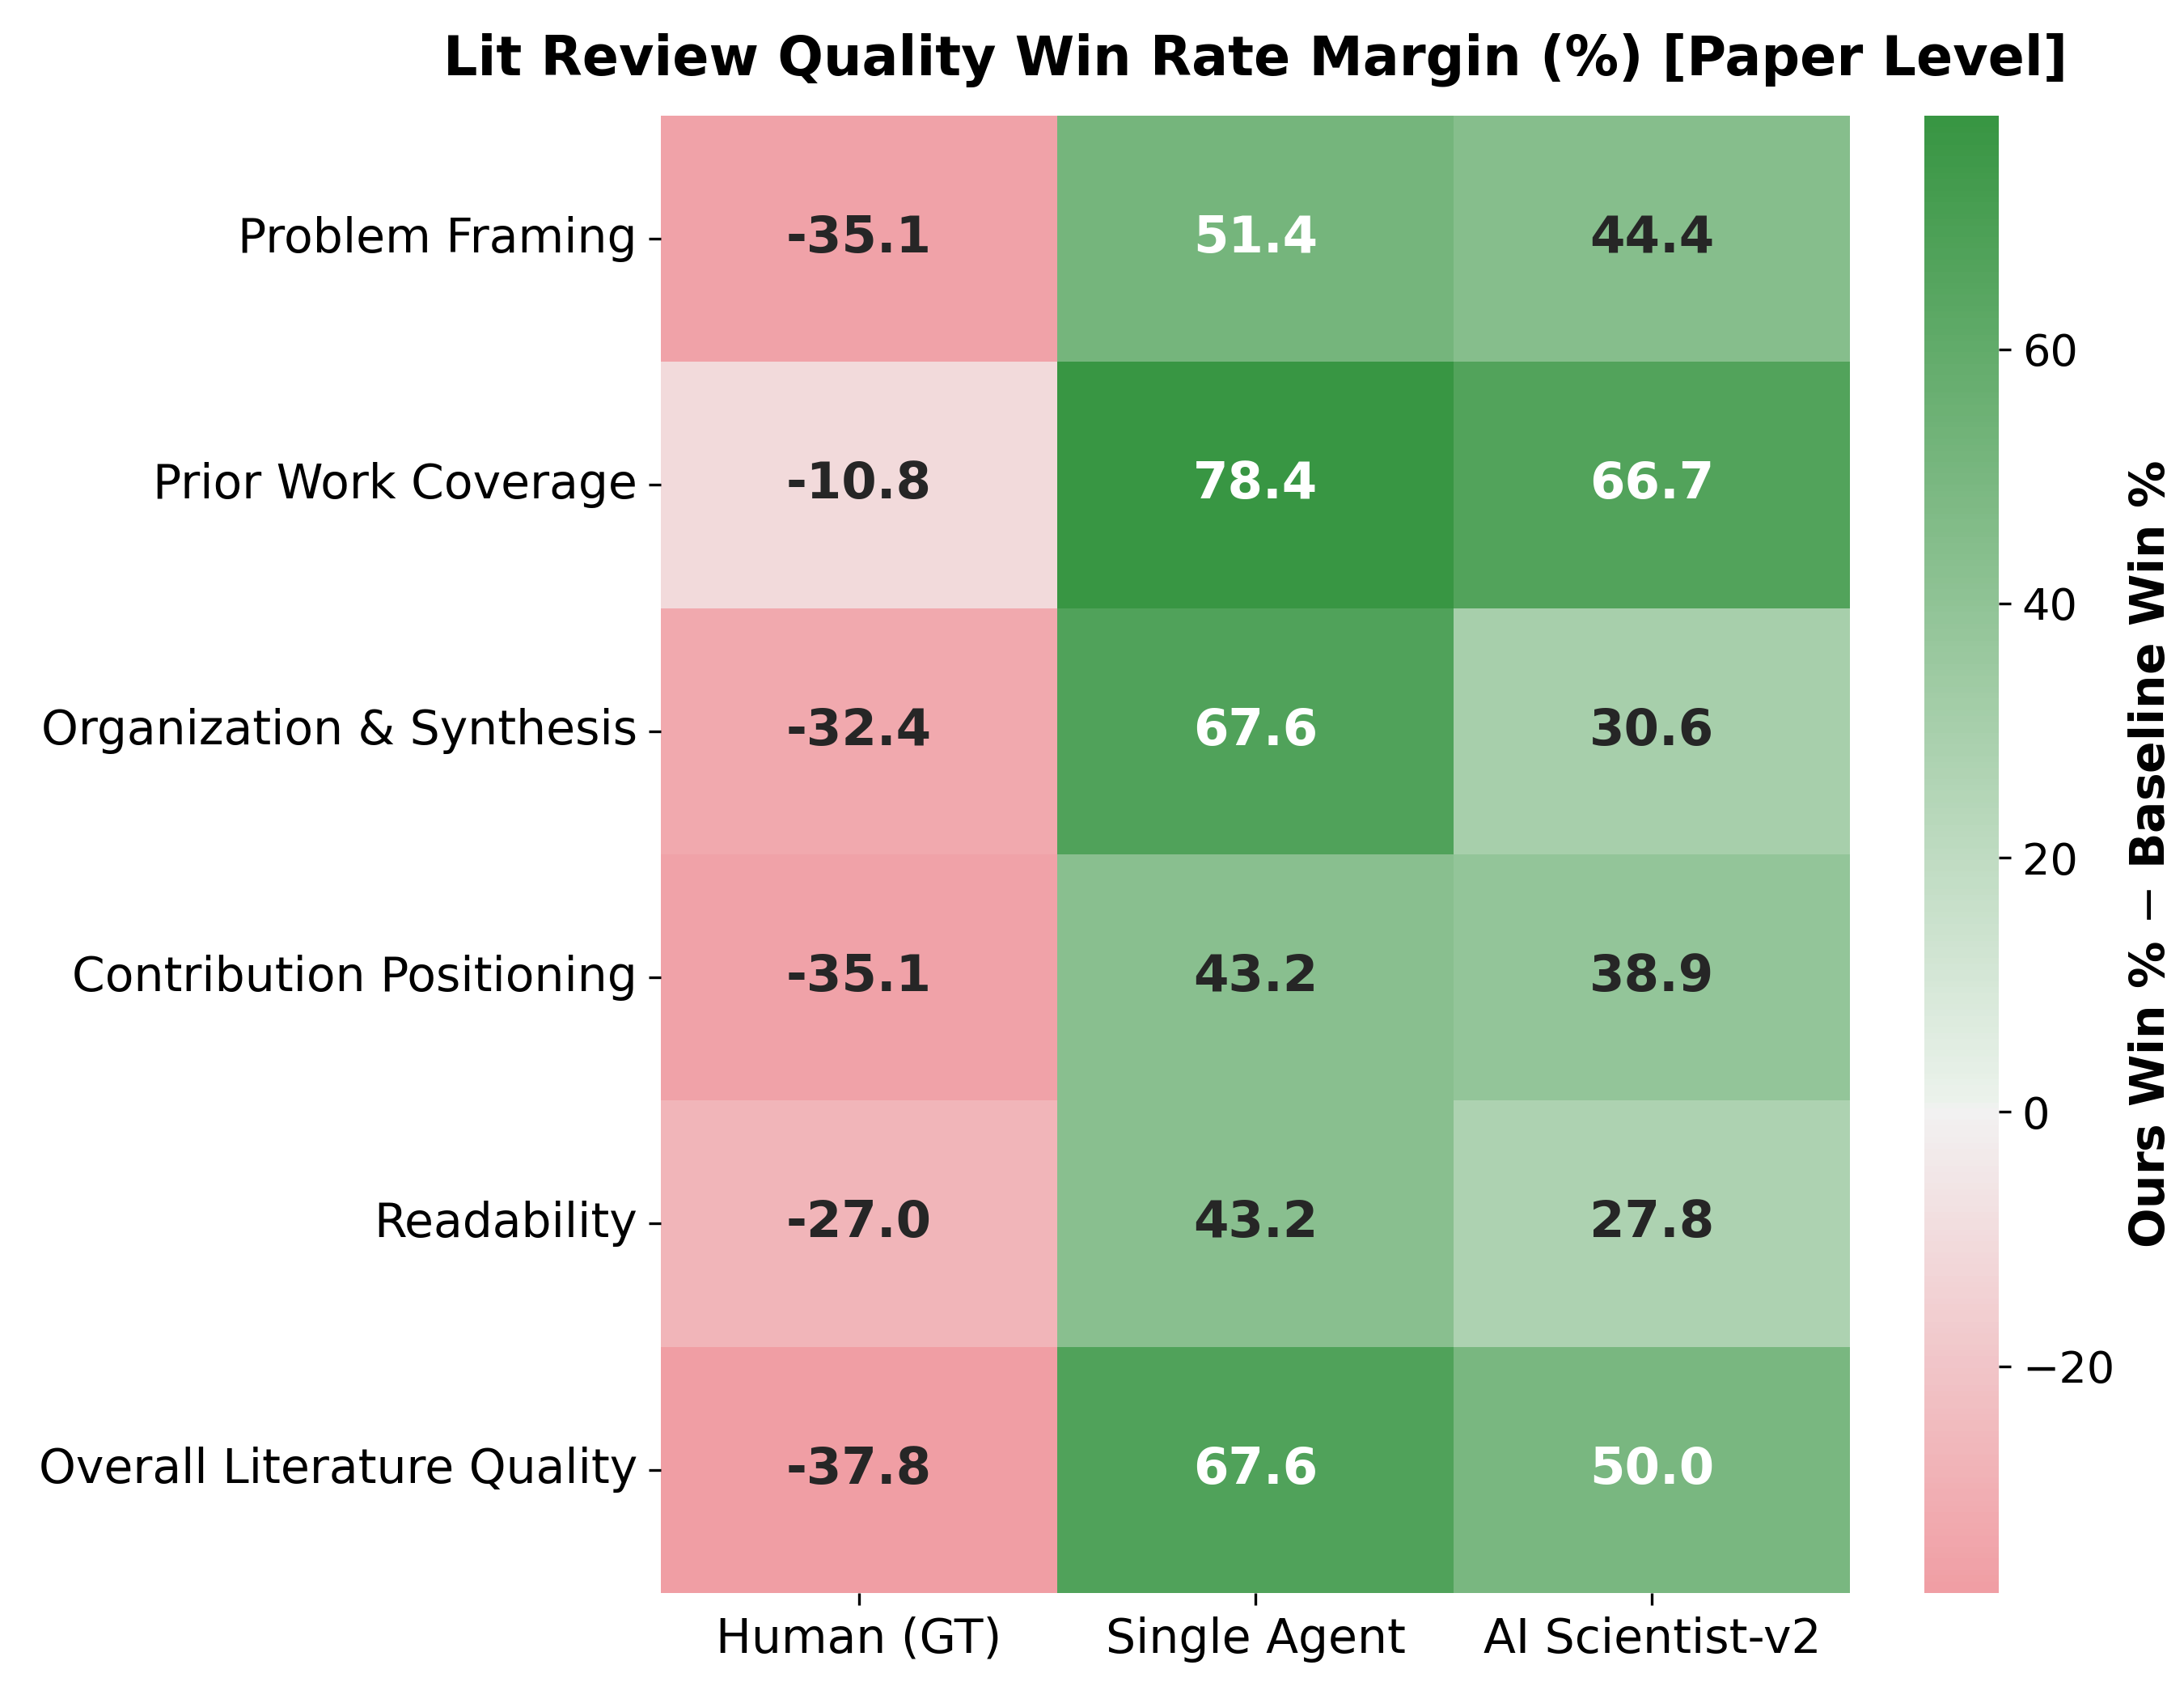
\includegraphics[width=\textwidth]{content/figures/human_eval_lit_heatmap.png}
    \caption{SxS Results: Literature Review Quality}
    \label{fig:human_eval_heatmap_lit}
  \end{subfigure}
  \hfill
  \begin{subfigure}[b]{0.48\textwidth}
    \centering
    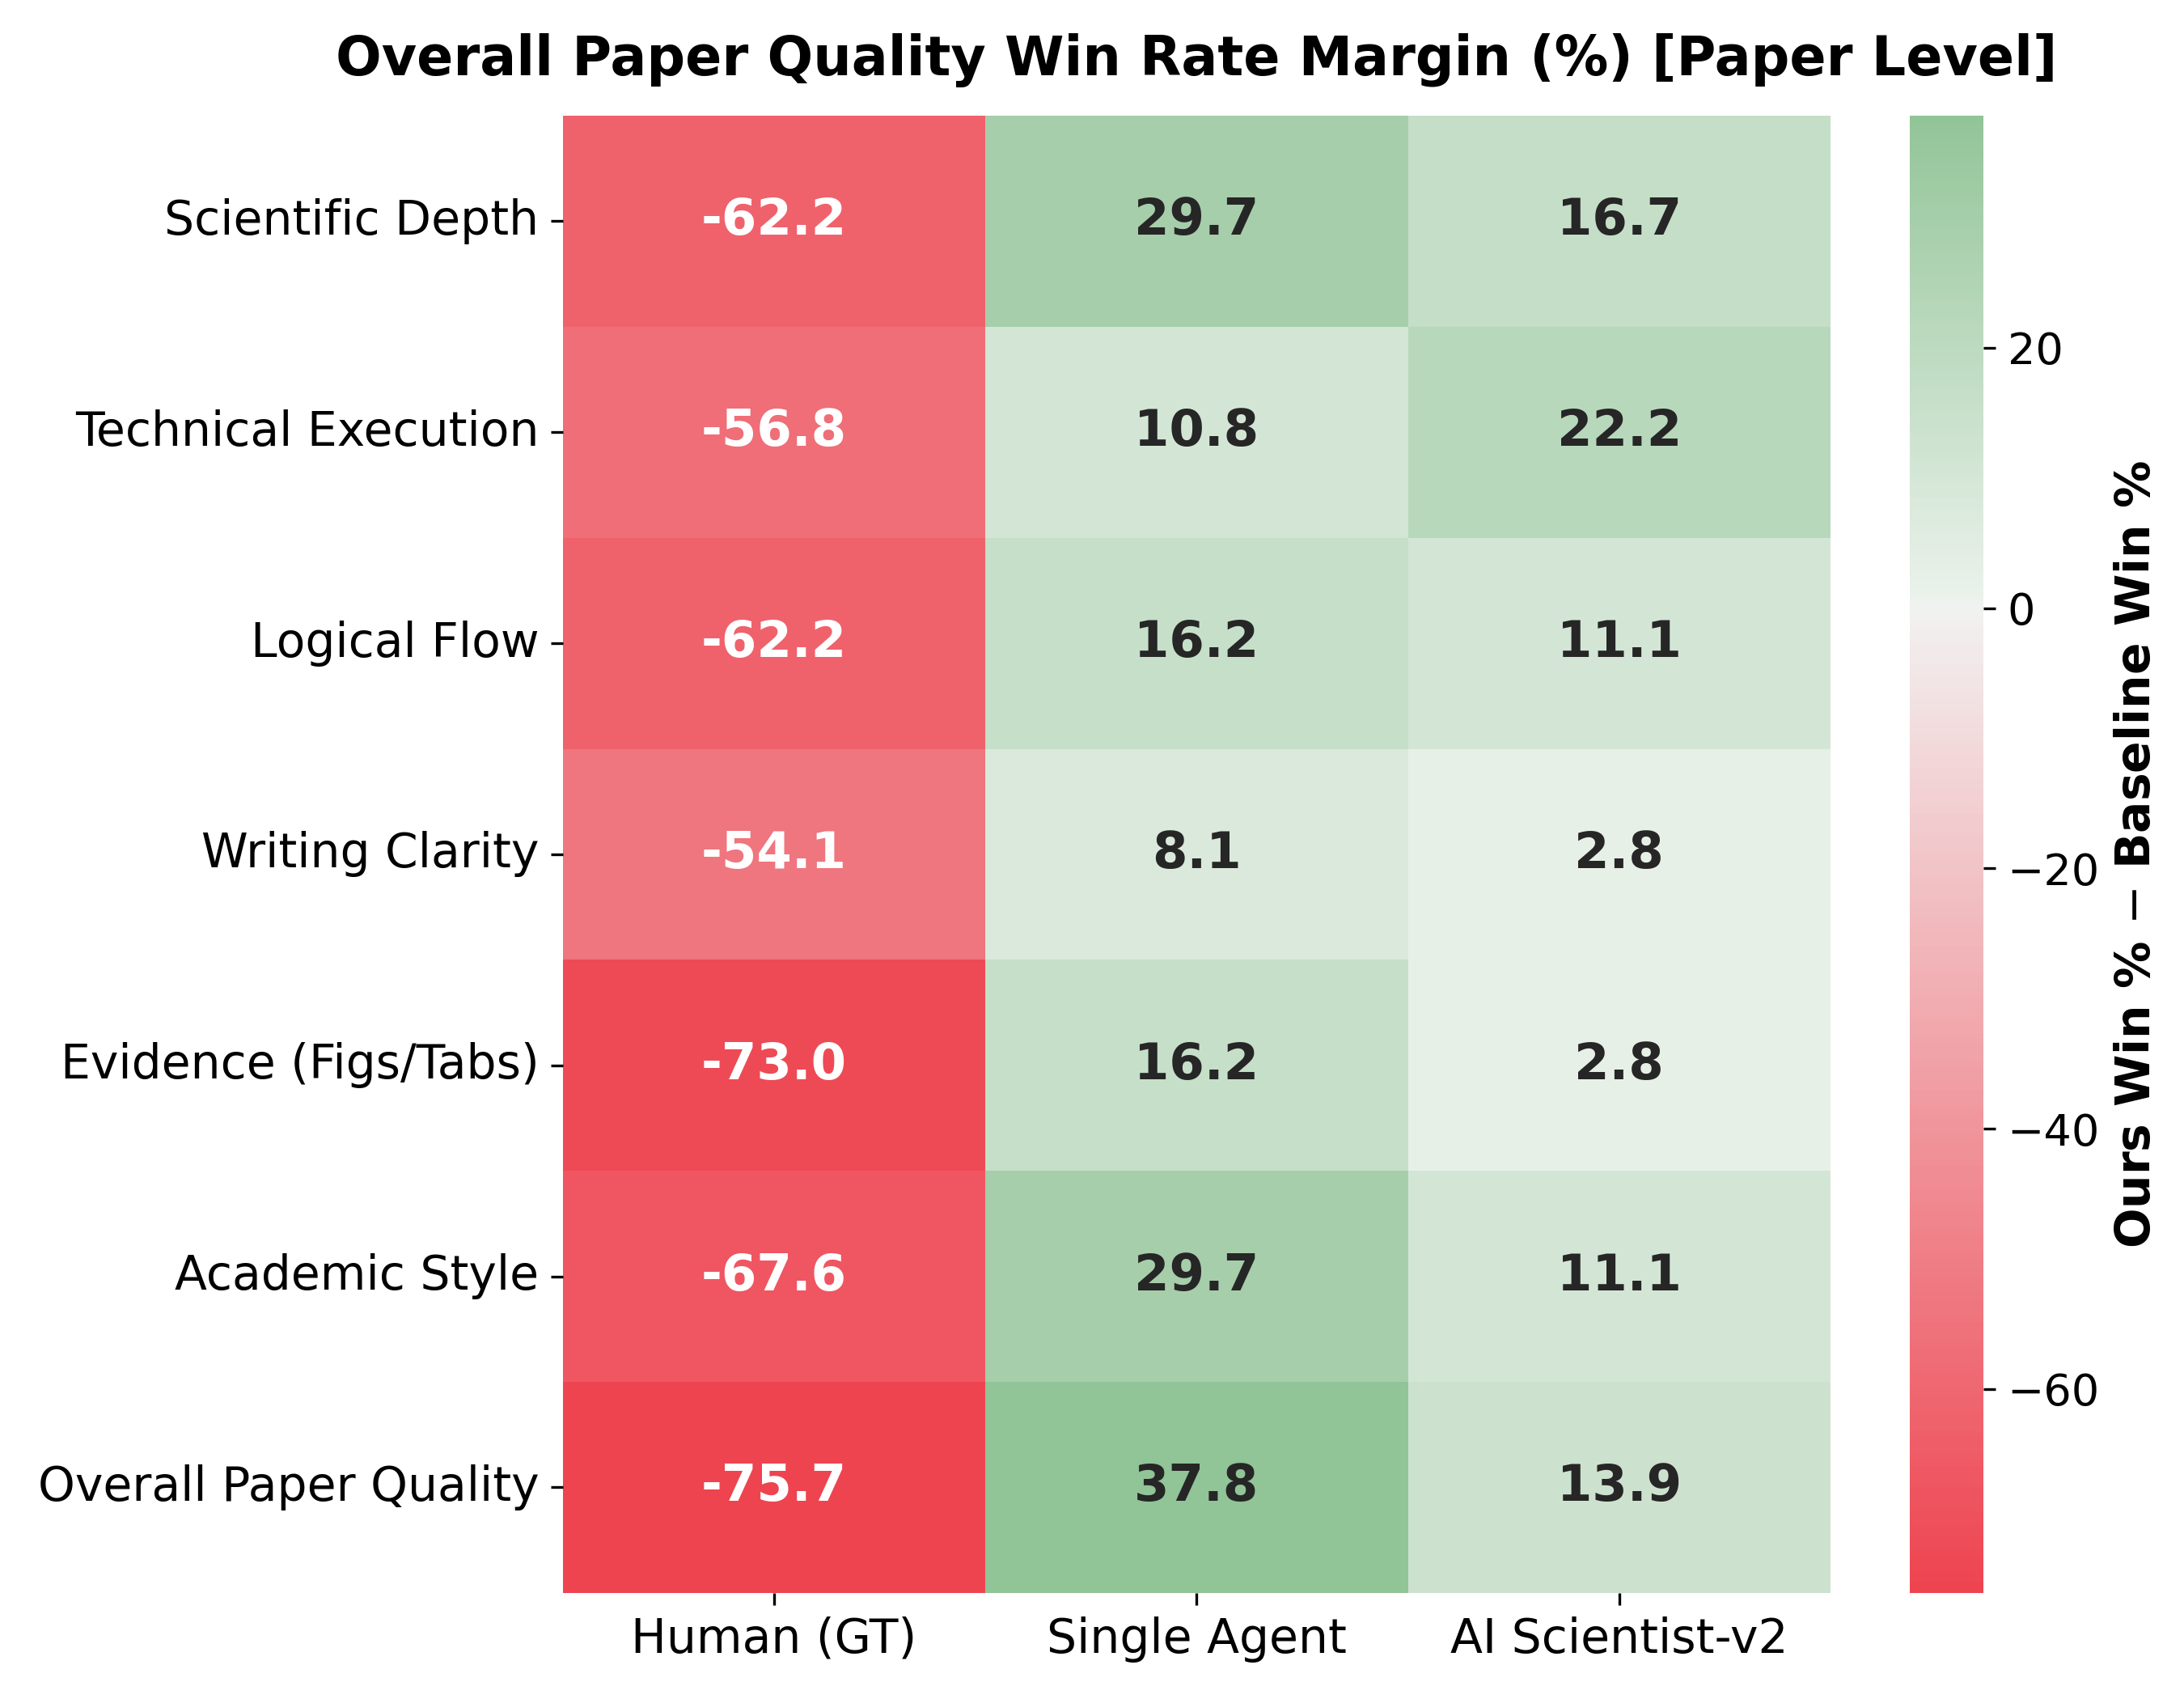
\includegraphics[width=\textwidth]{content/figures/human_eval_overall_heatmap.png}
    \caption{SxS Results: Overall Paper Quality}
    \label{fig:human_eval_heatmap_overall}
  \end{subfigure}
  \caption{\textbf{Human Side-by-Side (SxS) Evaluation Results.} Heatmaps display the win rate margin (\%) of \ourmethod{} against baselines across various evaluation dimensions. Positive values (green) favor our approach. \ourmethod{} consistently outperforms both AI baselines (Single Agent and AI Scientist-v2), though a quality gap remains compared to the human-written ground truth (GT).}
  \label{fig:human_eval_heatmaps_appendix}
\end{figure}

We developed a Streamlit interface (Figure~\ref{fig:human_eval_interface}) for blind SxS comparison of generated manuscripts. Annotators evaluated paper pairs on a 3-point scale (Win, Tie, Loss) across two aspects: (1) \textit{Literature Review Quality} (evaluating the \textit{Introduction} and \textit{Related Work}) based on problem framing, prior work coverage, synthesis, positioning, and readability; and (2) \textit{Overall Paper Quality} (evaluating the full manuscript) based on scientific depth, technical execution, logical flow, writing clarity, evidence presentation, and academic style. 

Eleven AI researchers completed 180 randomized, paired evaluations across 40 sampled papers from \ourdataset{} (120 unique paper pairs). For each evaluation, annotators answered 12 fine-grained diagnostic questions before making a final holistic judgment. As shown in Figure~\ref{fig:human_eval_heatmaps_appendix}, our approach, \ourmethod{}, systematically outperforms all AI baselines across every evaluation metric. While a quality gap remains when compared to the human-written papers (GT), \ourmethod{} achieves substantial win margins over all evaluated AI baselines in both literature review synthesis and overall paper quality.
\vspace{1em}

\begin{figure}[htbp]
  \centering
  \begin{subfigure}[b]{\textwidth}
    \centering
    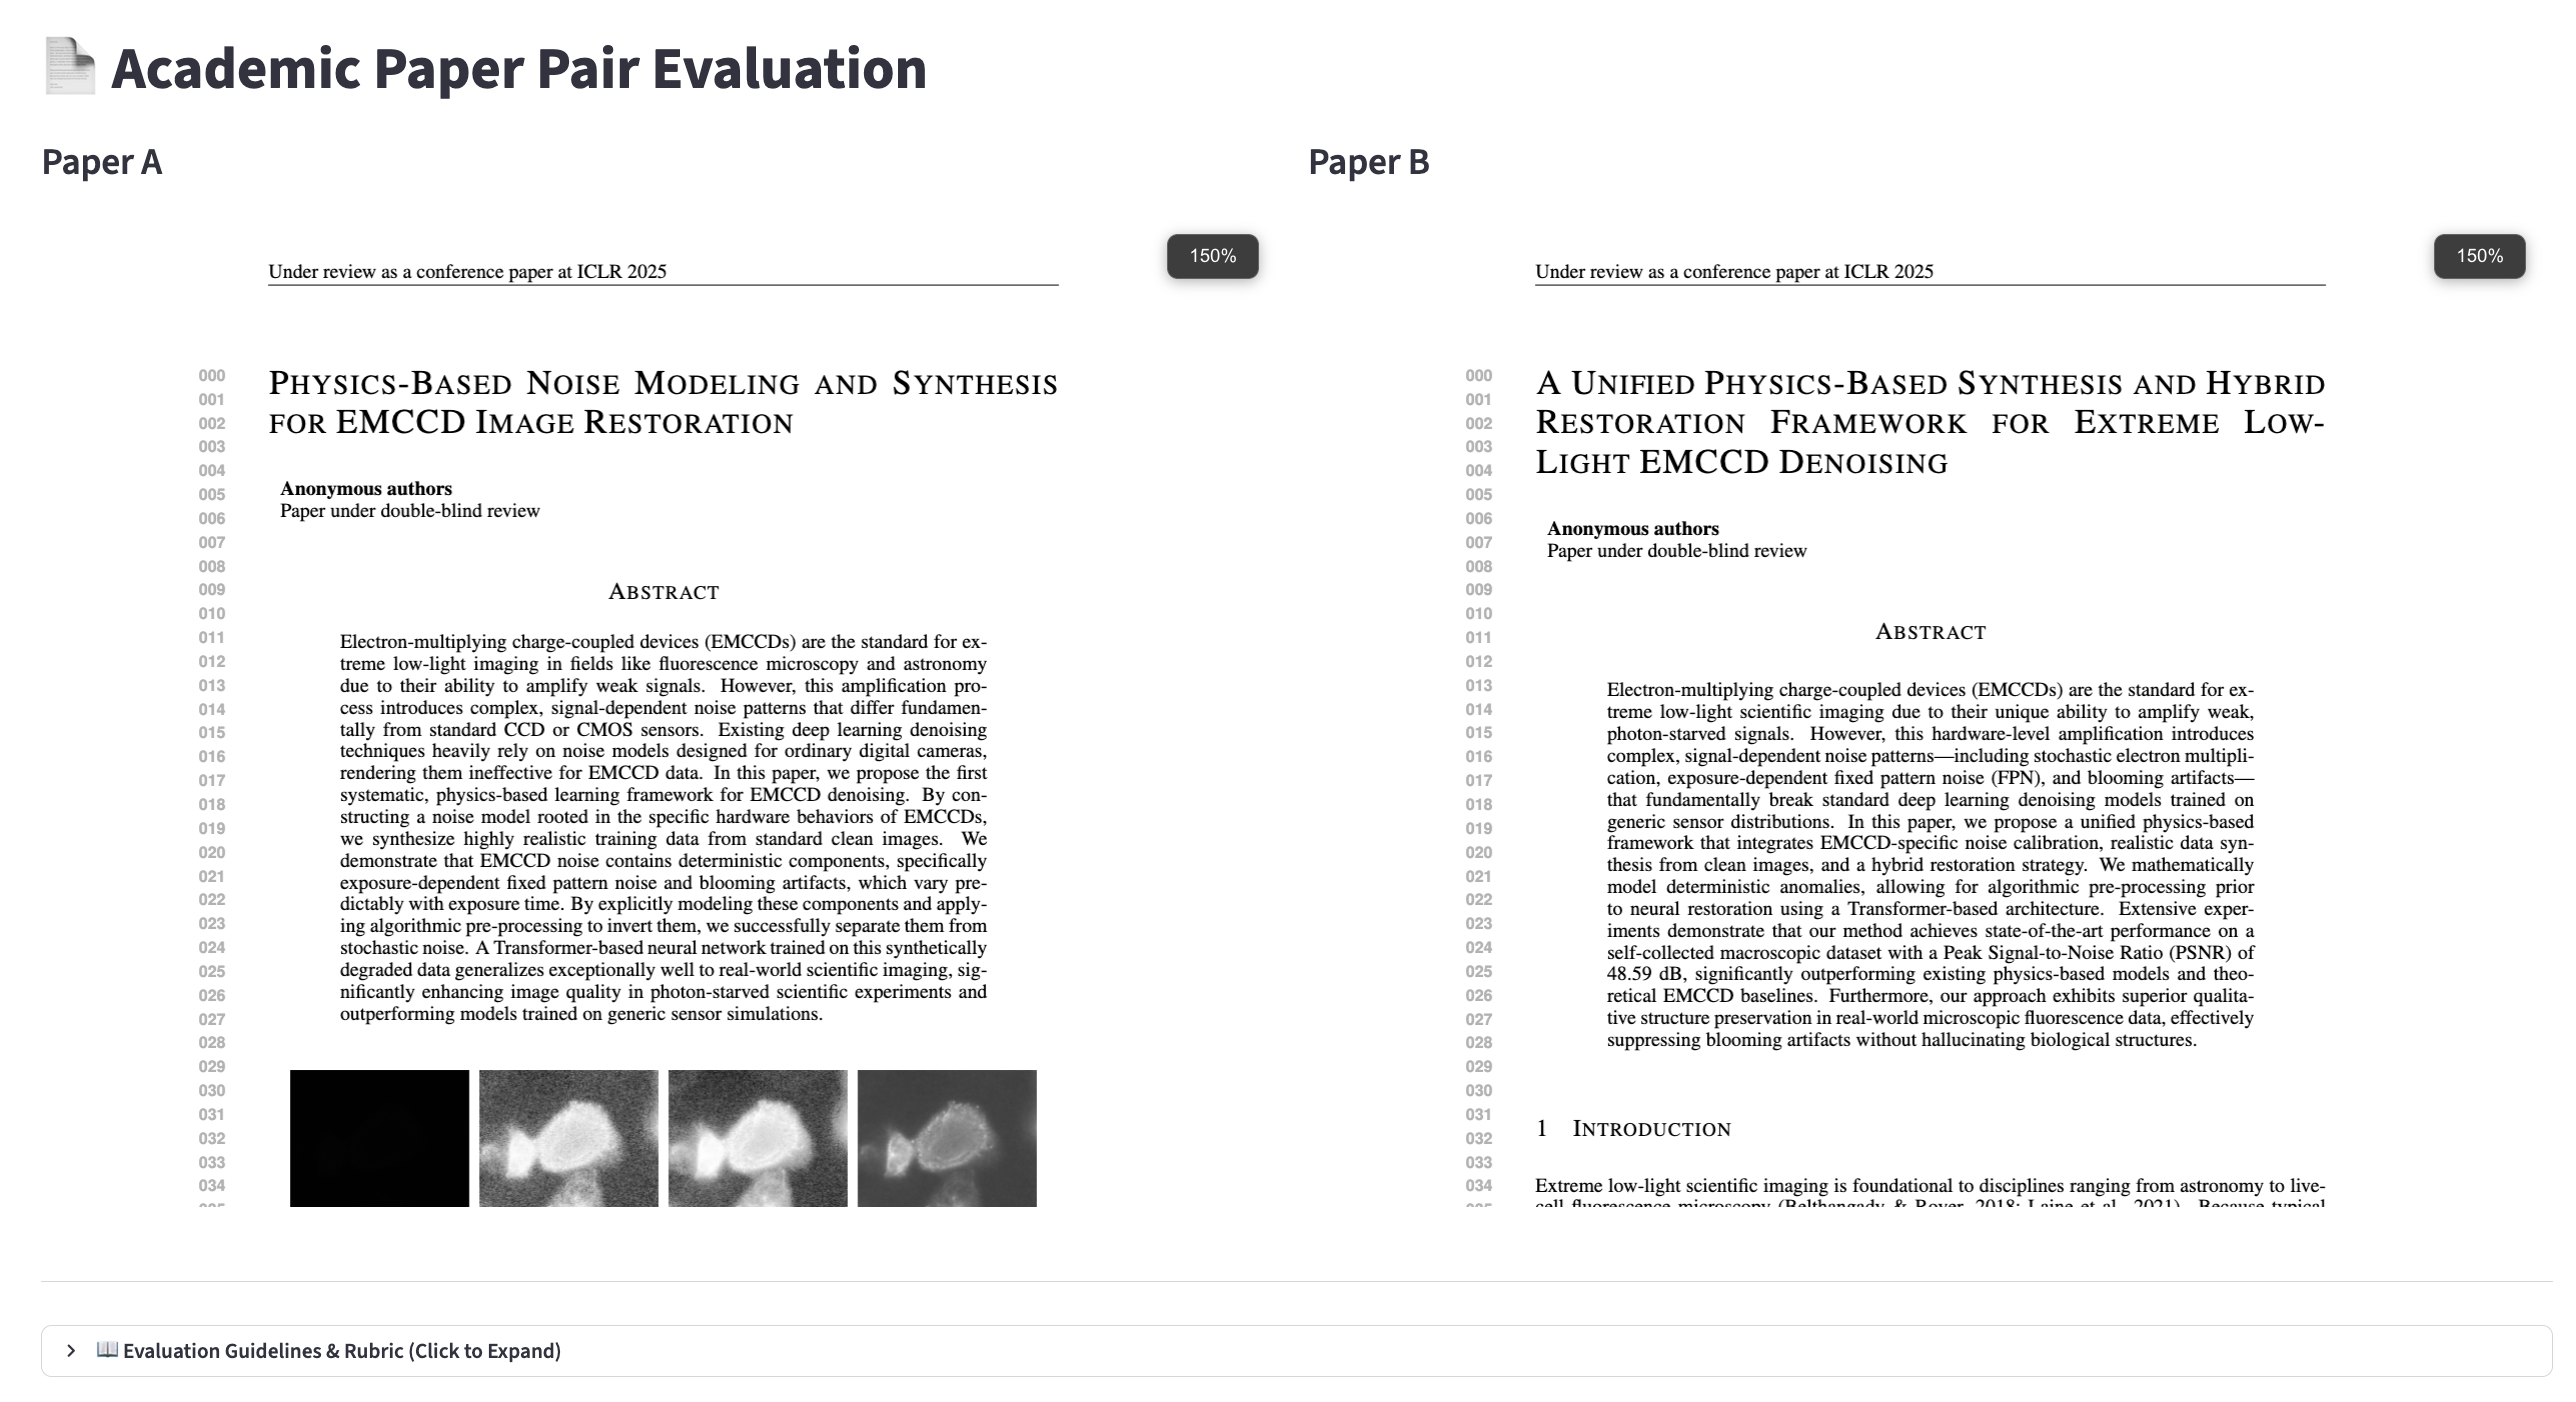
\includegraphics[width=0.8\linewidth]{content/figures/human_eval_ui_1.png}
    \caption{Side-by-Side Document View}
    \label{fig:human_eval_ui_top}
  \end{subfigure}
  
  \vspace{1em} % Adds vertical space between the two rows
  
  \begin{subfigure}[b]{\textwidth}
    \centering
    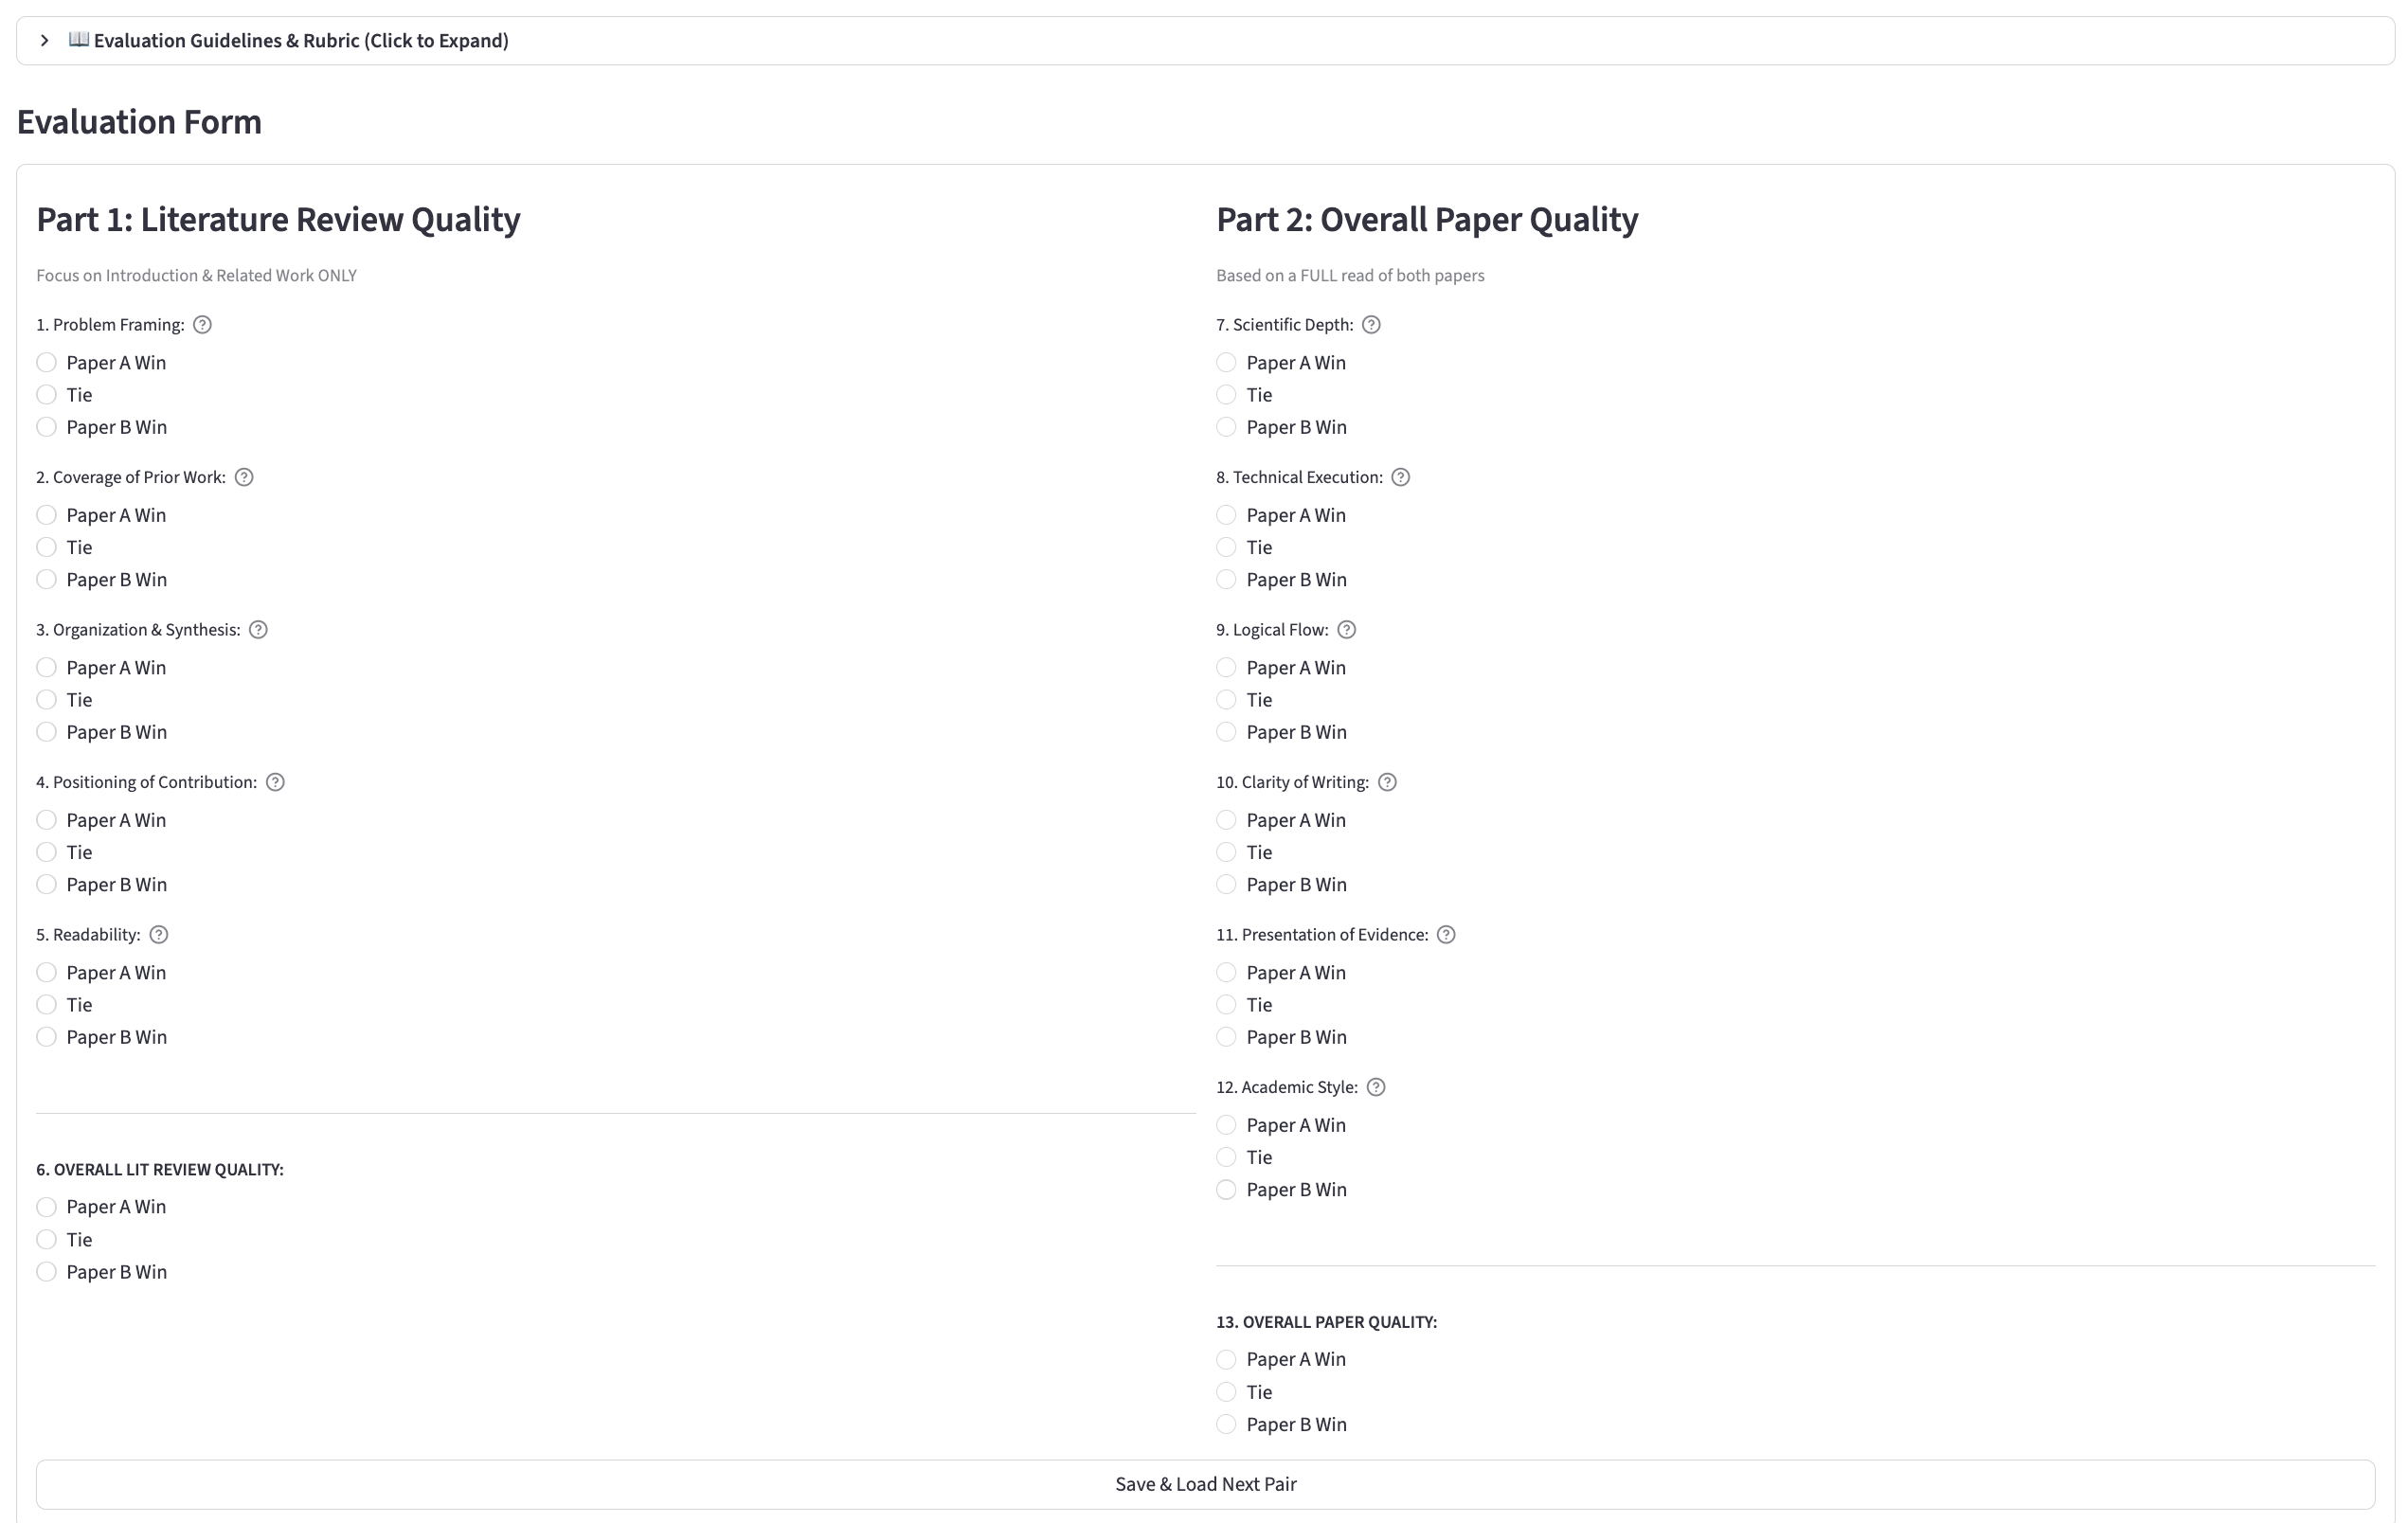
\includegraphics[width=0.75\linewidth]{content/figures/human_eval_ui_2.png}
    \caption{Evaluation Questionnaire}
    \label{fig:human_eval_ui_bottom}
  \end{subfigure}
  \caption{\textbf{Streamlit-based Human Evaluation Interface.} The custom UI displays two manuscripts side-by-side (a) and provides a fine-grained questionnaire alongside a final preference selection (b).}
  \label{fig:human_eval_interface}
\end{figure}

% ---------------------------------------------------------
% ---------------------------------------------------------

The detailed annotation guidelines and rubric provided to the human annotators are listed below:

\begin{humanevalbox}[Human Annotation Guidelines \& Rubric]
\textbf{General Rules}
\vspace{0.5em}
\begin{itemize}
    \item \textbf{Reading Scope:} 
    \begin{itemize}
        \item \textbf{Literature Review Quality} must be judged by reading the \textbf{Introduction and Related Work} sections \textit{only}.
        \item \textbf{Overall Paper Quality} must be judged based on a \textbf{full read} of both papers entirely.
    \end{itemize}
    \item \textbf{Ignore Templates and Metadata:} Some papers may include conference templates (e.g., CVF headers), watermarks, or text indicating prior publication. \textbf{Additionally, some papers may list author names while others are anonymized for review.} Please completely ignore these artifacts. Evaluations must be based purely on the intrinsic quality of the text and research, not the templates, perceived prestige, or author identities.
    \item Evaluate each paper independently before comparing them.
    \item \textbf{Do not} base your decision solely on paper length or verbosity.
\end{itemize}

\vspace{1em}
\noindent\textbf{Literature Review Quality (Focus on Introduction \& Related Work)}
\vspace{0.5em}
\begin{itemize}
    \item \textbf{Motivation:} Does it clearly explain the problem, why it matters, and the gap in existing work?
    \item \textbf{Coverage:} Is the overview of prior research relevant and complete?
    \item \textbf{Synthesis:} Does it organize and group related work logically, rather than just blindly listing papers?
    \item \textbf{Positioning:} Does it clearly explain how \textit{this} paper differs from existing methods?
    \item \textbf{Readability:} Is the text concise, clear, and easy to follow?
\end{itemize}

\vspace{1em}
\noindent\textbf{Overall Paper Quality (Holistic Review)}
\vspace{0.5em}
\begin{itemize}
    \item \textbf{Scientific Depth:} Are the theoretical foundations, justifications, and experimental setups rigorous?
    \item \textbf{Execution:} Is the methodology implemented innovatively and effectively?
    \item \textbf{Logical Flow:} Does the paper transition smoothly from Abstract to Conclusion?
    \item \textbf{Clarity:} Is the writing precise and free of repetitive fluff or ambiguity?
    \item \textbf{Evidence:} Are figures, tables, and results cleanly integrated and referenced in the text?
    \item \textbf{Style:} Does it maintain a polished, consistent, professional academic tone?
\end{itemize}
\end{humanevalbox}



% ---------------------------------------------------------
% ---------------------------------------------------------